3.1 Convolutional Neural Network (CNN)
\hfill \

A Convolutional Neural Network (CNN) is a type of deep learning algorithm specifically designed for image processing and recognition tasks. Compared to alternative classification models, CNNs require less preprocessing as they can automatically learn hierarchical feature representations from raw input images[7].
\centering
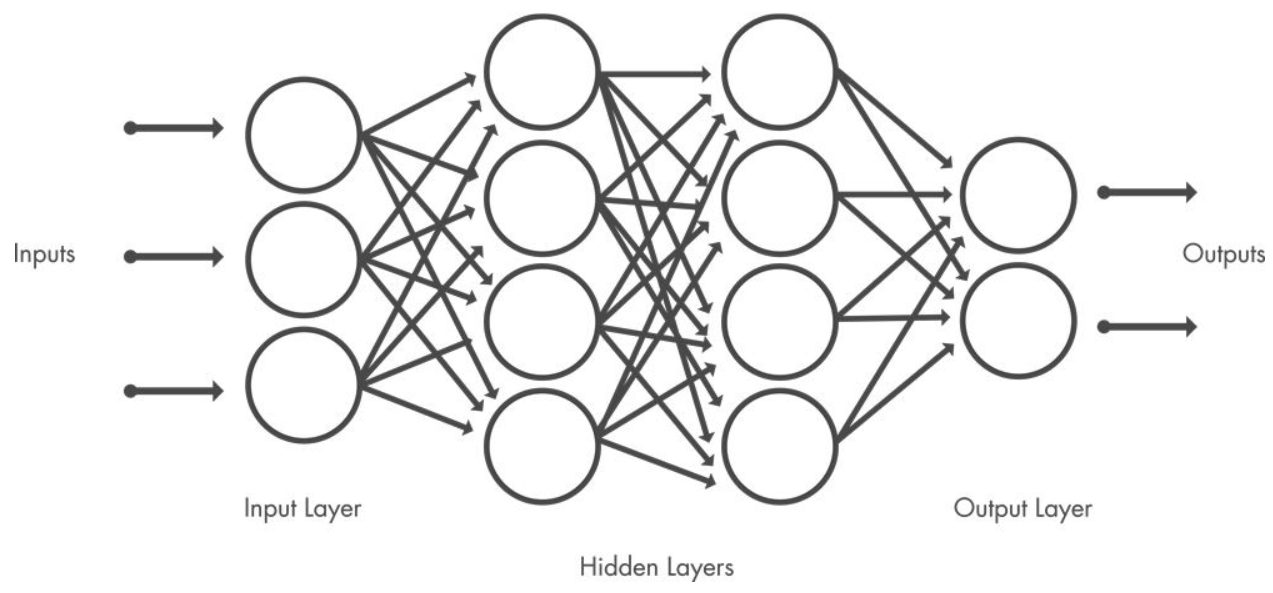
\includegraphics[width=.5\textwidth]{Cnn.PNG}
\hfill \break

3.2. EfficientNet B0
\hfill \break
EfficientNet architecture consists of seven blocks which are shown in different colours. The basic building block of EfficientNet-B0 is a mobile inverted bottleneck convolution (MBConv), while each MBConv block is shown with the corresponding kernel filter size [6]. The figure below shows the different block

\centering
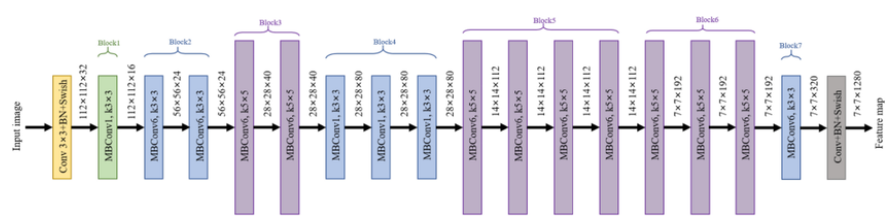
\includegraphics[width=.5\textwidth]{EfficientNet.PNG}
\hfill \break







